\section{Prototipos de interfaz de usuario}
\label{sec:prototipos_interfaz}

El diseño de la interfaz de usuario materializa los requisitos funcionales y las reglas de negocio descritas en los apartados anteriores, transformando los contratos de datos en flujos de interacción intuitivos y accesibles. Para la concepción visual de Colivi se adoptó la herramienta de diseño vectorial Figma, desarrollando un sistema de diseño (\emph{Design System}) fundamentado en la metodología \emph{Atomic Design} de Brad Frost.

Este enfoque modular garantiza coherencia estética y ergonomía cognitiva a través de una paleta cromática sobria, una retícula responsiva basada en múltiplos de 8 píxeles y una jerarquía tipográfica sin serifa. A continuación se detallan las pantallas clave que componen el núcleo operativo de la plataforma, abordando desde la captación y búsqueda de inmuebles hasta la convivencia comunitaria cotidiana.

\subsection{Acceso, autenticación y bienvenida}

La pantalla de acceso (figura \ref{fig:prot_login}) actúa como punto de entrada a los servicios protegidos de Colivi. El diseño minimiza la fricción inicial permitiendo al usuario autenticarse mediante credenciales locales (correo electrónico y contraseña) o delegar la identidad mediante el protocolo federado Google OAuth (\hyperref[tab:requisitos-funcionales]{RF-02} y \hyperref[tab:requisitos-funcionales]{RF-03}).

\begin{figure}[H]
    \centering
    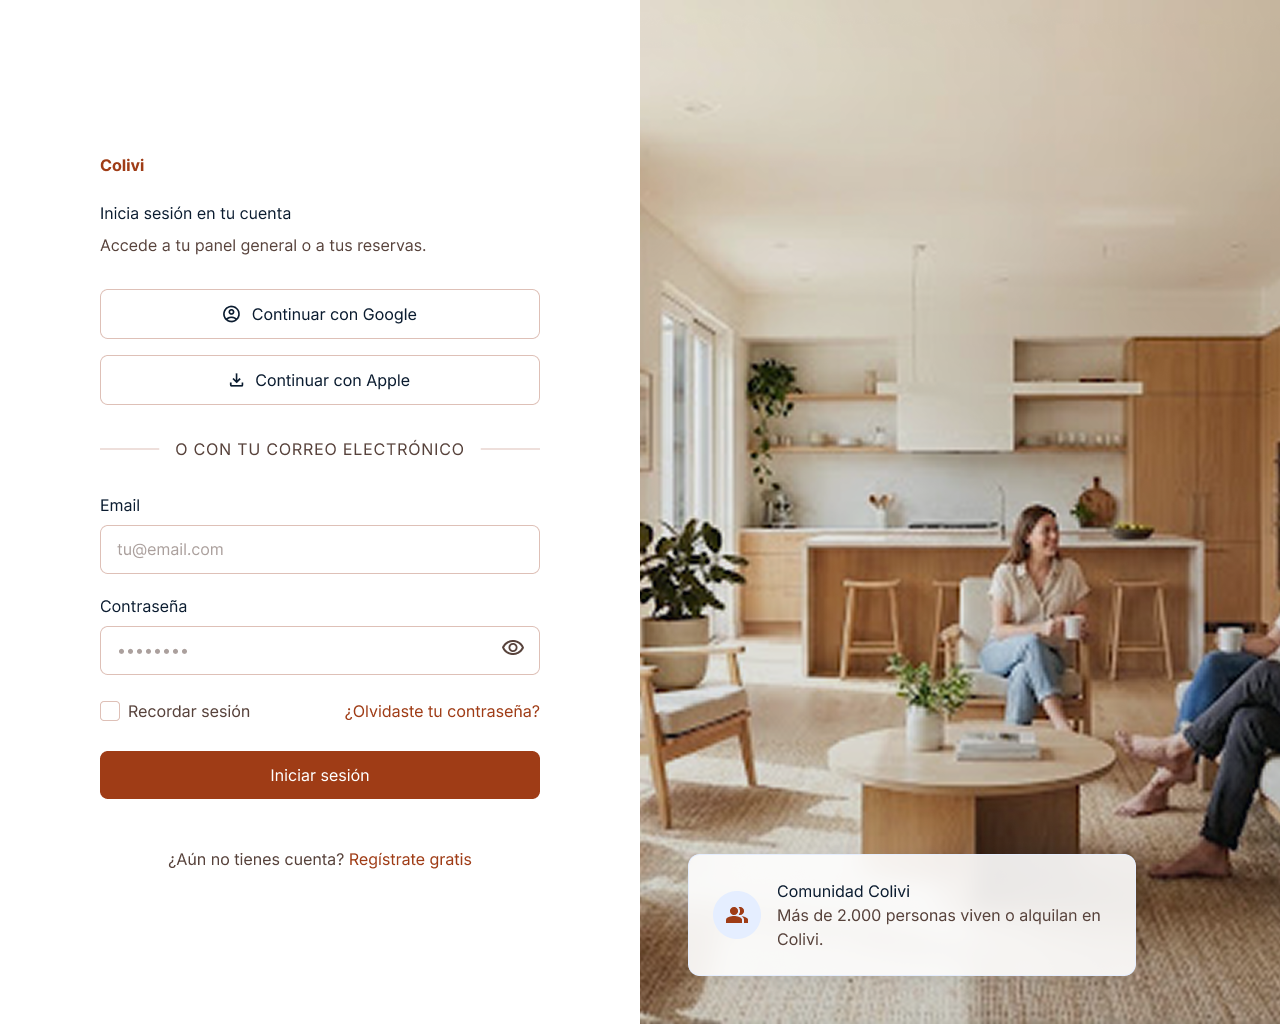
\includegraphics[width=0.75\textwidth]{AnalisisFuncional/img/prot_login.png}
    \caption{Prototipo de la interfaz de inicio de sesión y autenticación federada. Elaboración propia}
    \label{fig:prot_login}
\end{figure}

El formulario incorpora validación reactiva en tiempo real para evitar envíos erróneos y proporciona accesos directos al restablecimiento de contraseñas olvidadas y al registro de nuevas cuentas. En conformidad con el requisito \hyperref[tab:requisitos-no-funcionales]{RNF-05}, los mensajes de retroalimentación ante credenciales inválidas o cuentas bloqueadas se presentan mediante alertas contextuales claras que no comprometen la seguridad del sistema.

\subsection{Exploración geográfica e interactiva de alojamientos}

Para facilitar la localización de vivienda a los estudiantes, el explorador de alojamientos (figura \ref{fig:prot_mapa}) articula una vista combinada con mapa interactivo y listado filtrable (\hyperref[tab:requisitos-funcionales]{RF-16} y \hyperref[tab:requisitos-funcionales]{RF-17}).

\begin{figure}[H]
    \centering
    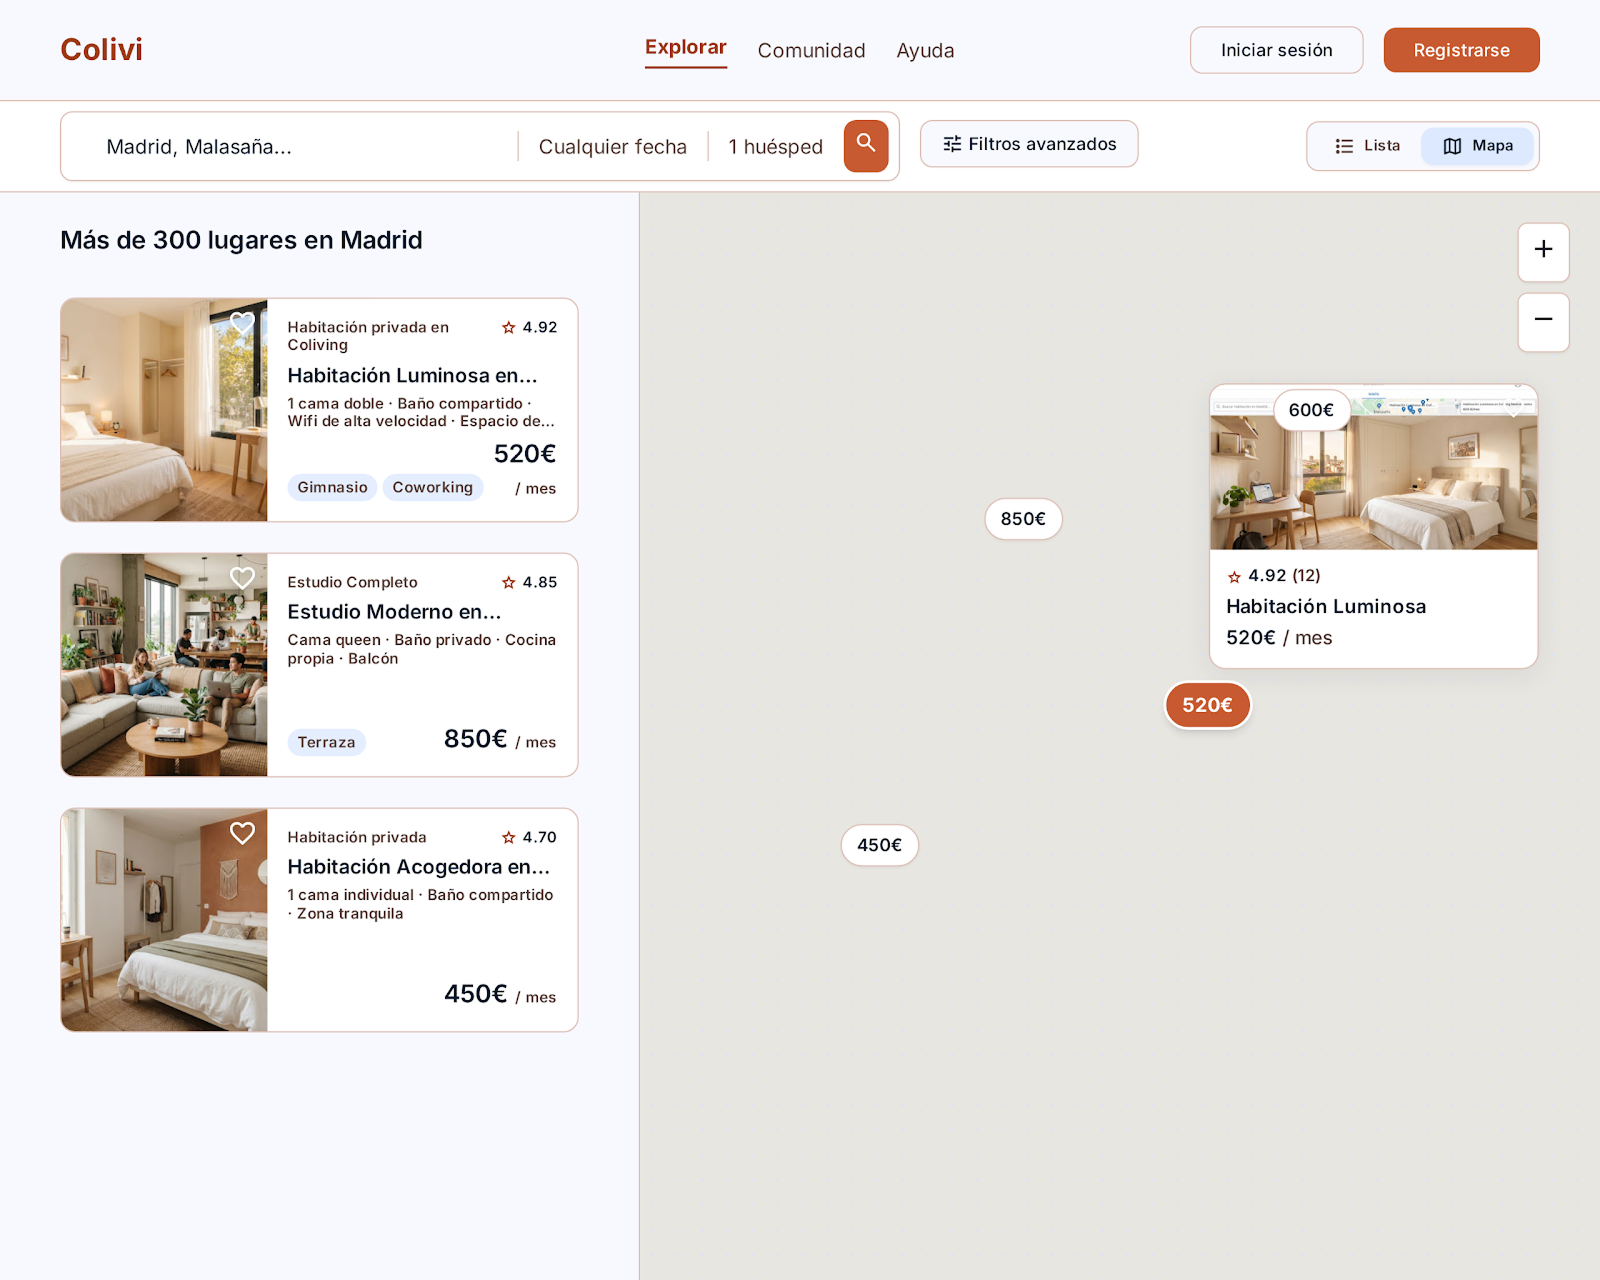
\includegraphics[width=0.85\textwidth]{AnalisisFuncional/img/prot_mapa.png}
    \caption{Prototipo del explorador interactivo con mapas y filtros combinados. Elaboración propia}
    \label{fig:prot_mapa}
\end{figure}

La pantalla integra un visor cartográfico basado en Leaflet y OpenStreetMap enriquecido con las siguientes capacidades ergonómicas:
\begin{itemize}
    \item \textbf{Filtrado multicriterio:} Barra lateral con controles deslizantes para rango de precios, selector de tipología (habitación individual o piso completo), número de dormitorios y comodidades (\emph{amenities}) como conexión a internet, calefacción o ascensor.
    \item \textbf{Agrupación de marcadores (\emph{Clustering}):} Los inmuebles cercanos se agrupan numéricamente para preservar la legibilidad del mapa ante altas densidades de oferta.
    \item \textbf{Tarjetas de previsualización rápida:} Al seleccionar un pin en el mapa, se despliega una tarjeta flotante con el carrusel de fotografías, el precio mensual y la valoración media acumulada, agilizando la decisión previa a la navegación en profundidad.
\end{itemize}

\subsection{Catálogo detallado y reserva de alojamiento}

La vista de detalle de alojamiento (figura \ref{fig:prot_alojamientos}) ofrece una exposición integral de las características físicas, legales y económicas de la propiedad (\hyperref[tab:requisitos-funcionales]{RF-18} y \hyperref[tab:requisitos-funcionales]{RF-32}).

\begin{figure}[H]
    \centering
    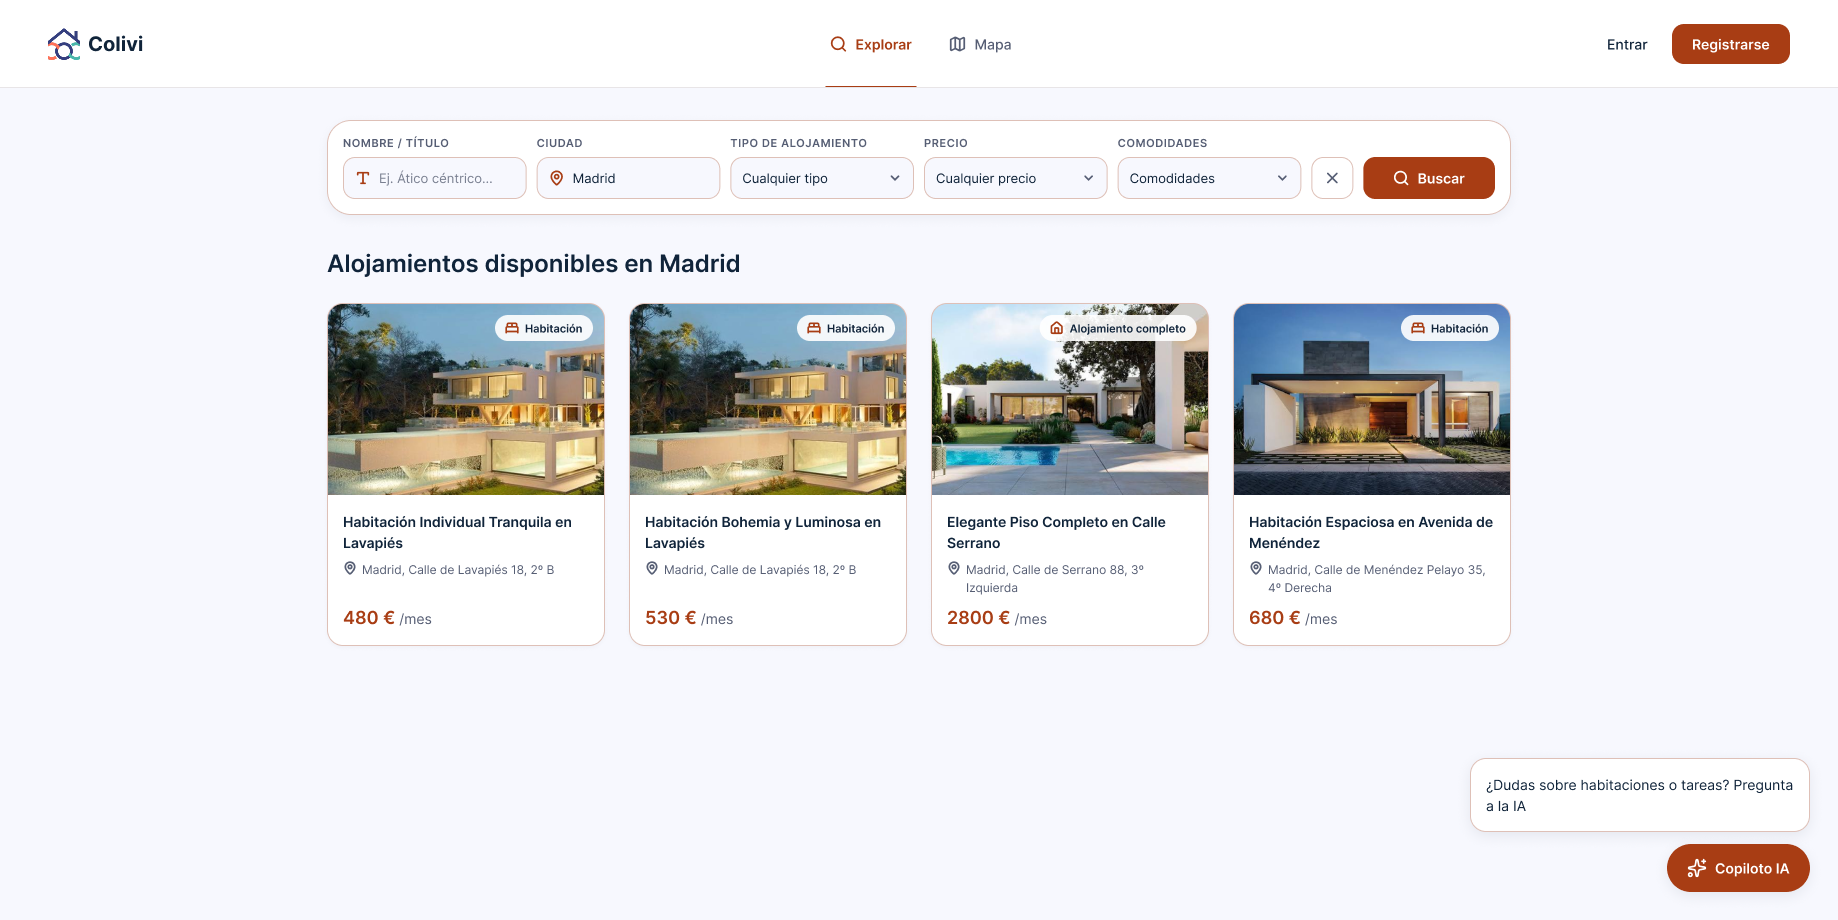
\includegraphics[width=0.95\textwidth]{AnalisisFuncional/img/prot_alojamientos.png}
    \caption{Prototipo de la ficha detallada de inmueble y panel de contratación. Elaboración propia}
    \label{fig:prot_alojamientos}
\end{figure}

La maqueta organiza la información en bloques semánticos definidos:
\begin{itemize}
    \item \textbf{Galería multimedia de alta resolución:} Presentación de las fotografías alojadas en la CDN con navegación modal interactiva y diferenciación entre zonas comunes y dormitorios privados.
    \item \textbf{Condiciones contractuales transparentes:} Desglose explícito de la renta mensual, depósito de fianza requerido, políticas de cancelación y fecha límite de disponibilidad.
    \item \textbf{Perfil del anfitrión y reputación comunitaria:} Visualización de la puntuación media obtenida y comentarios de inquilinos precedentes (\hyperref[tab:requisitos-funcionales]{RF-29}), reduciendo la asimetría informativa.
    \item \textbf{Panel flotante de reserva (\emph{Sticky Booking Card}):} Selector de intervalo temporal que calcula automáticamente el coste total e inicia el flujo de solicitud al pulsar sobre la acción principal.
\end{itemize}

\subsection{Panel de control de comunidades de convivencia}

El módulo de convivencia doméstica centraliza los pisos compartidos a los que pertenece el usuario. La pantalla de listado de hogares (figura \ref{fig:prot_lista_hogares}) permite transicionar ágilmente entre diferentes viviendas presentes o archivadas (\hyperref[tab:requisitos-funcionales]{RF-40} y \hyperref[tab:requisitos-funcionales]{RF-49}).

\begin{figure}[H]
    \centering
    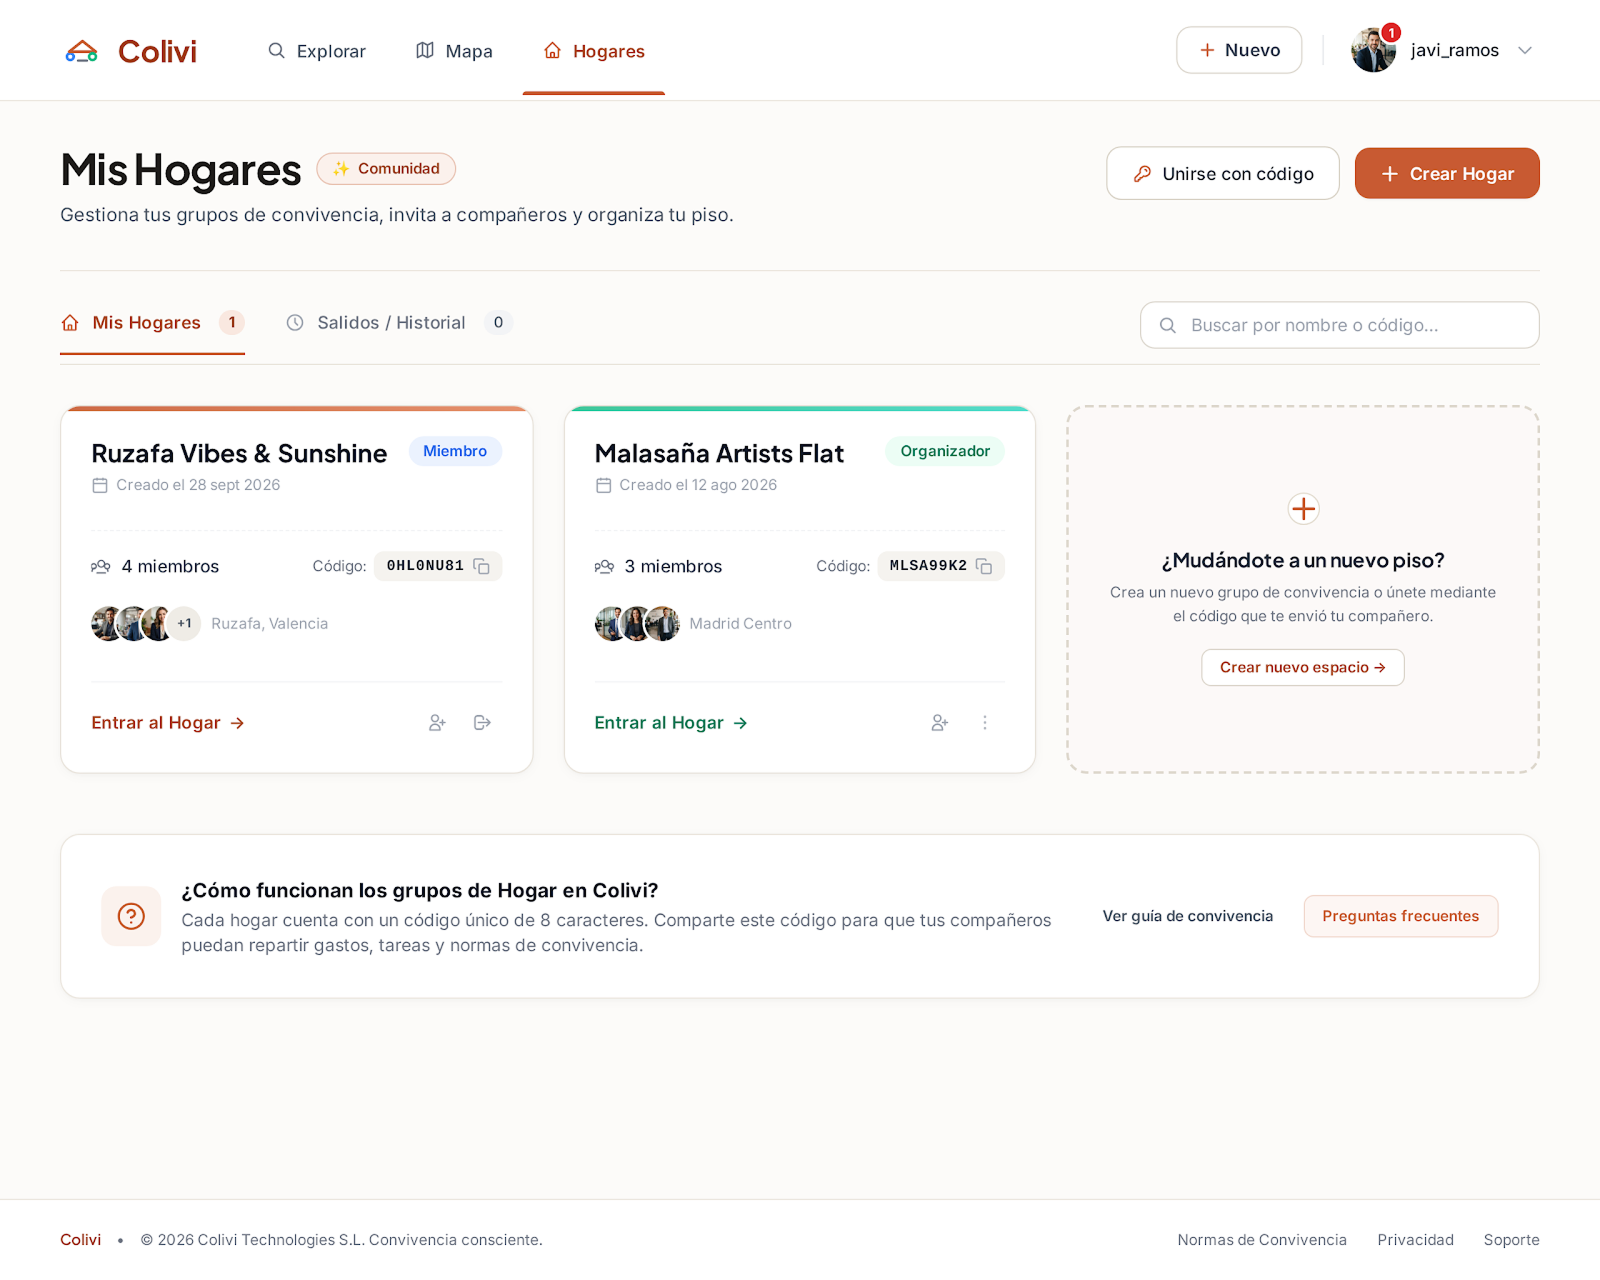
\includegraphics[width=0.85\textwidth]{AnalisisFuncional/img/prot_lista_hogares.png}
    \caption{Prototipo del panel centralizado de hogares y gestión de convivencias. Elaboración propia}
    \label{fig:prot_lista_hogares}
\end{figure}

Cada tarjeta de hogar sintetiza el pulso actual de la vivienda: la dirección física, los avatares e identidades cromáticas de los compañeros de piso (\hyperref[tab:requisitos-funcionales]{RF-43}), el balance personal acumulado y los indicadores de tareas pendientes. Desde este mismo panel se habilitan dos acciones estratégicas: crear un nuevo espacio de convivencia (\hyperref[tab:requisitos-funcionales]{RF-39}) o unirse a un piso preexistente introduciendo un código de invitación seguro (\hyperref[tab:requisitos-funcionales]{RF-42}).

\subsection{Gestión y liquidación de gastos compartidos}

La gestión financiera comunitaria se materializa en la pantalla de balances y gastos del hogar (figura \ref{fig:prot_gastos}), diseñada para eliminar la ambigüedad en los repartos económicos (\hyperref[tab:requisitos-funcionales]{RF-50} a \hyperref[tab:requisitos-funcionales]{RF-55}).

\begin{figure}[H]
    \centering
    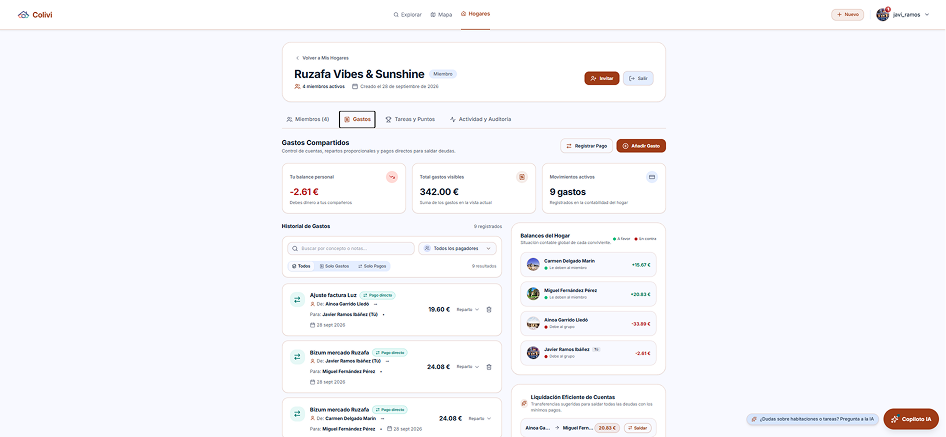
\includegraphics[width=0.85\textwidth]{AnalisisFuncional/img/prot_gastos.png}
    \caption{Prototipo del módulo contable y liquidación de deudas compartidas. Elaboración propia}
    \label{fig:prot_gastos}
\end{figure}

La interfaz presenta un resumen ejecutivo superior con el saldo neto del usuario (verde para crédito a favor, rojo para deuda pendiente). A continuación, desglosa:
\begin{itemize}
    \item \textbf{Transferencias sugeridas:} Cálculo optimizado que minimiza el número de transacciones bancarias necesarias para saldar las cuentas globales de la vivienda.
    \item \textbf{Historial cronológico auditado:} Listado de tickets y facturas con indicación del pagador original, el criterio de partición aplicado (a partes iguales o porcentual) y los miembros involucrados.
    \item \textbf{Acción de liquidación inmediata:} Mecanismo rápido para registrar pagos efectuados en metálico o mediante pasarelas externas, garantizando que el saldo retorne a cero antes de cualquier salida del hogar (\hyperref[tab:requisitos-funcionales]{RF-56}).
\end{itemize}

\subsection{Planificación y cuadrante de tareas domésticas}

El mantenimiento higiénico y operativo del inmueble se articula mediante el planificador de tareas (figura \ref{fig:prot_calendario_tareas}), combinando una vista en calendario con un cuadrante de asignaciones por turno (\hyperref[tab:requisitos-funcionales]{RF-57} a \hyperref[tab:requisitos-funcionales]{RF-61}).

\begin{figure}[H]
    \centering
    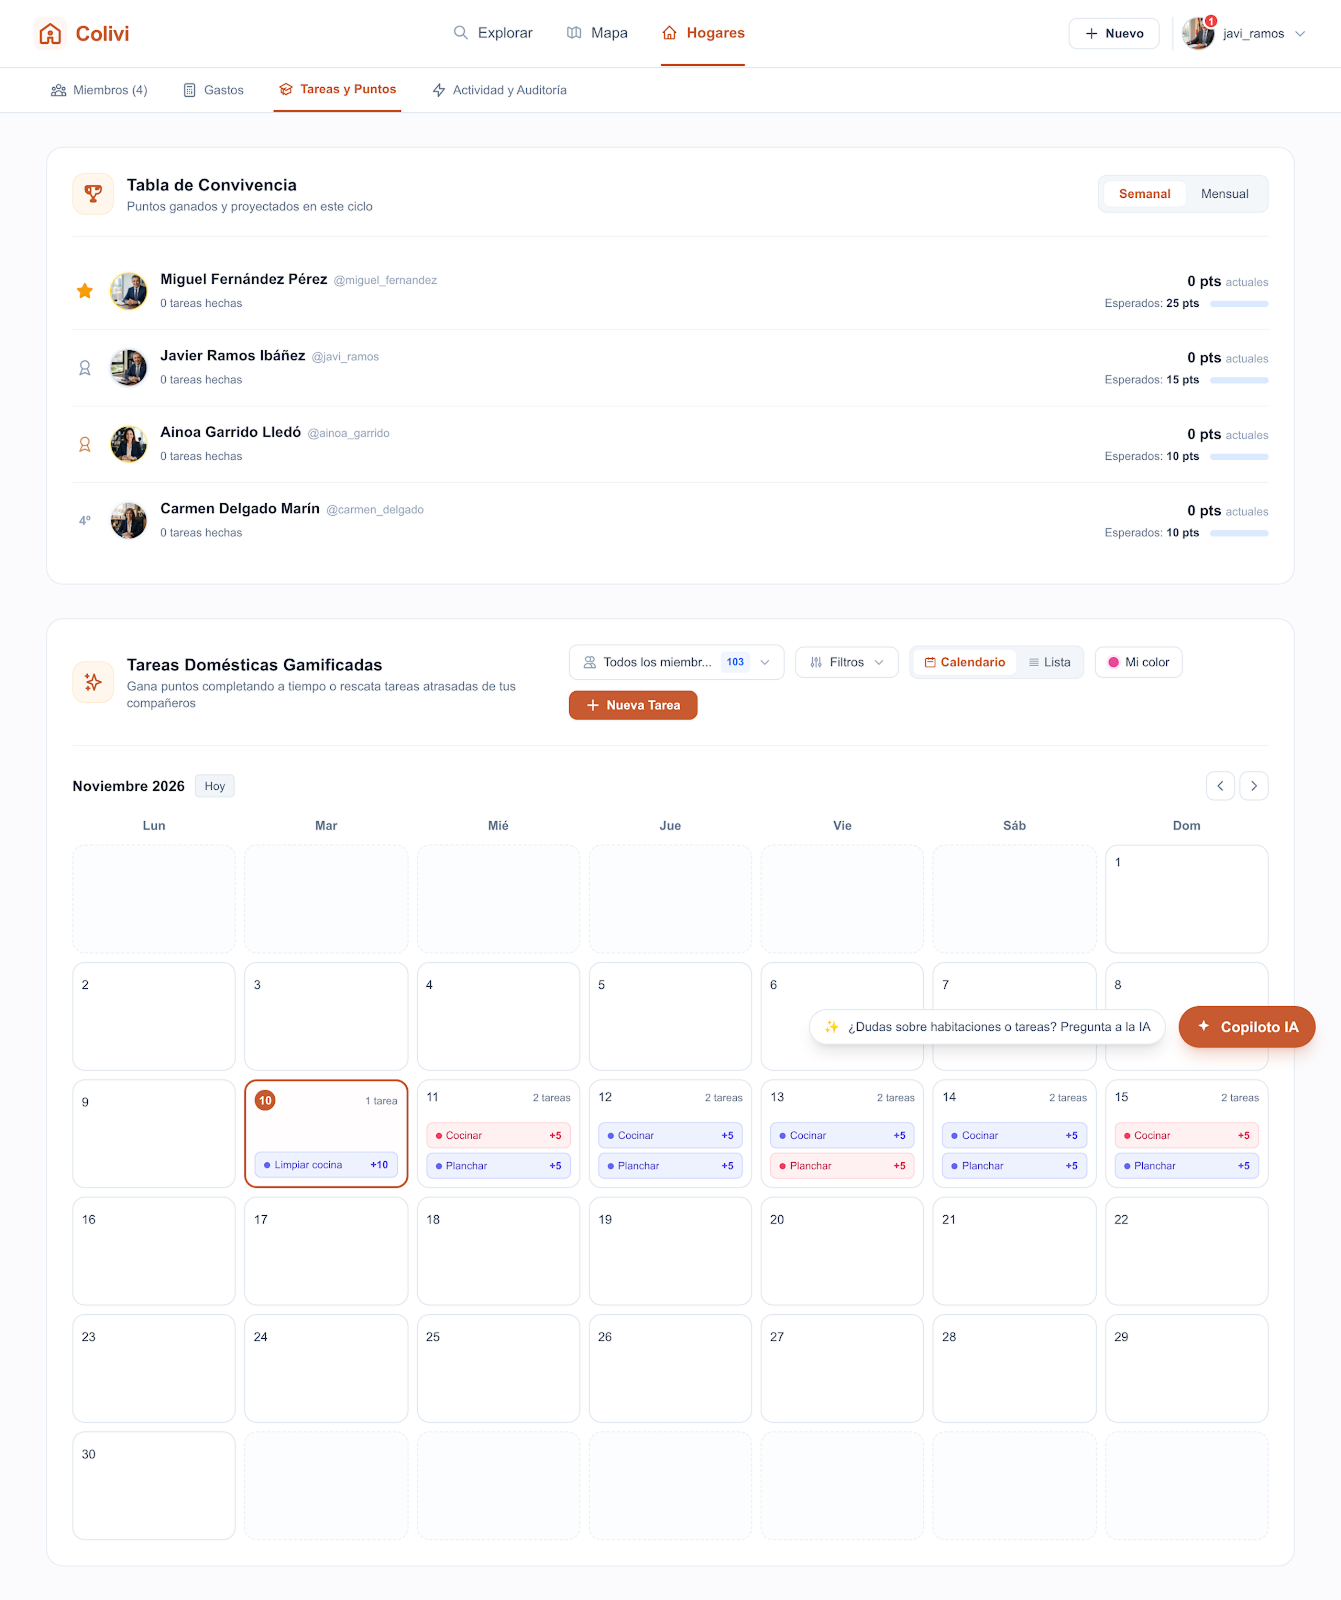
\includegraphics[width=0.65\textwidth]{AnalisisFuncional/img/prot_calendario_tareas.png}
    \caption{Prototipo del calendario y cuadrante rotativo de tareas domésticas. Elaboración propia}
    \label{fig:prot_calendario_tareas}
\end{figure}

El diseño fomenta la transparencia y la corresponsabilidad mediante:
\begin{itemize}
    \item \textbf{Codificación visual por estados:} Marcado diferenciado para tareas pendientes, completadas a tiempo y retrasadas, facilitando la auditoría visual rápida.
    \item \textbf{Turnos rotativos automáticos:} Representación del algoritmo \emph{Round-Robin} que alterna semanal o mensualmente a los responsables de labores críticas (limpieza de cocina, baños, reciclaje).
    \item \textbf{Funcionalidad de rescate voluntario:} Permite a cualquier compañero asumir y completar una labor vencida de otro miembro (\hyperref[tab:requisitos-funcionales]{RF-61}), previniendo tensiones en la convivencia.
\end{itemize}

